\documentclass[11pt]{beamer}
\usetheme{Warsaw}
\usepackage[utf8]{inputenc}
\usepackage{natbib}
\usepackage{amsmath}
\usepackage{graphicx}
\usepackage{subcaption}
\usepackage{tikz}
\usepackage{hyperref}
\setbeamertemplate{footline}[frame number]

\hypersetup{
    colorlinks=true,
    linkcolor=white,
    filecolor=magenta,      
    urlcolor=blue,
}


\title{Projet PSTALN}
\subtitle{Prédiction des \textit{morphy}}
\author{Cléa Han, Yanis Labeyrie et Adrien Zabban}
\date{15 janvier 2024}

\begin{document}

\maketitle

\begin{frame}{Le but: prédire les \textit{morphy}}
    \begin{figure}[b]
        \centering
        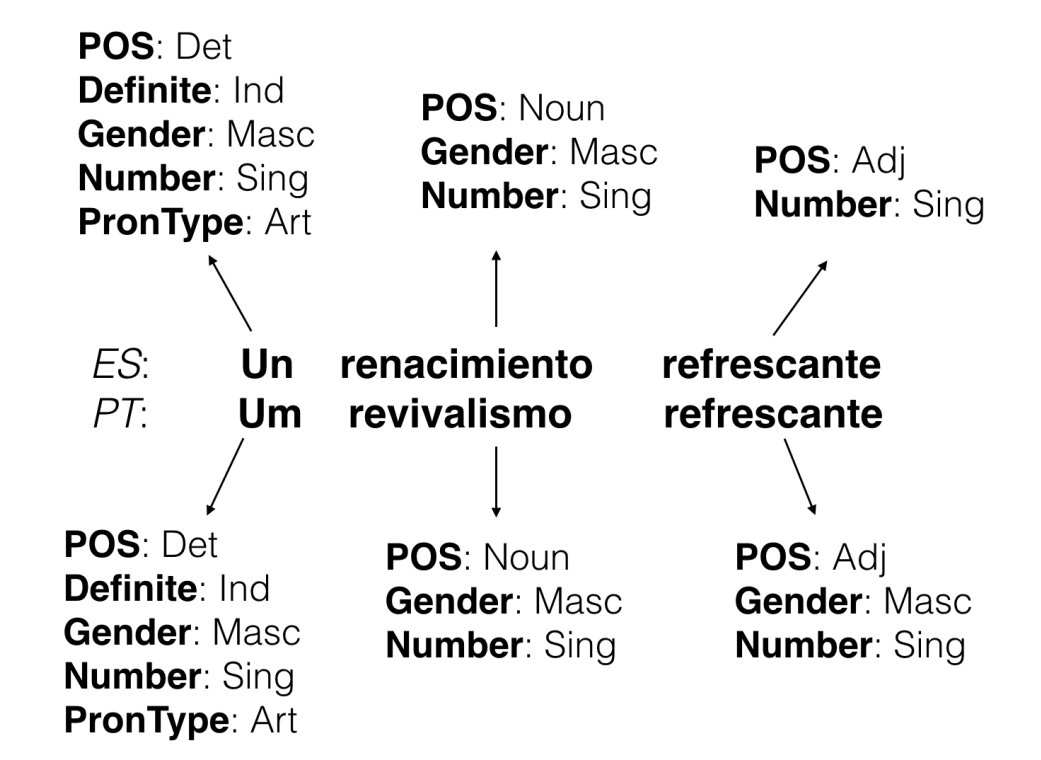
\includegraphics[width=0.8\textwidth]{morphy.png}
        % 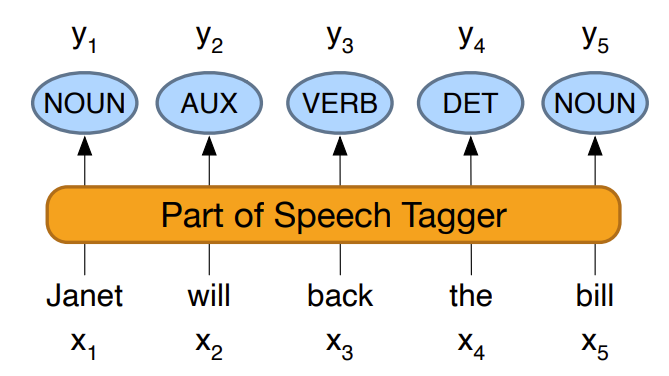
\includegraphics[width=0.40\textwidth]{pos.png}
        \caption{Tag morphologique d'une phrase portugaise et sa traduction en espagnol.}
    \end{figure}
\end{frame}

\begin{frame}{Les Données: Le dataset}
    Nous avons utilisé le dataset Universal Dependencies 2.13.

    Le dataset en français contient:
    \begin{itemize}
        \item 47498 phrases
        \item 849476 mots
        \item 76048 mots uniques
    \end{itemize}

    On a recensé:
    \begin{itemize}
        \item 19 classes \textit{pos}.
        \item 28 classes \textit{morphy}, avec un nombre de possibilités entre 2 et 13
    \end{itemize}
\end{frame}

\begin{frame}
    \begin{figure}
        \centering
        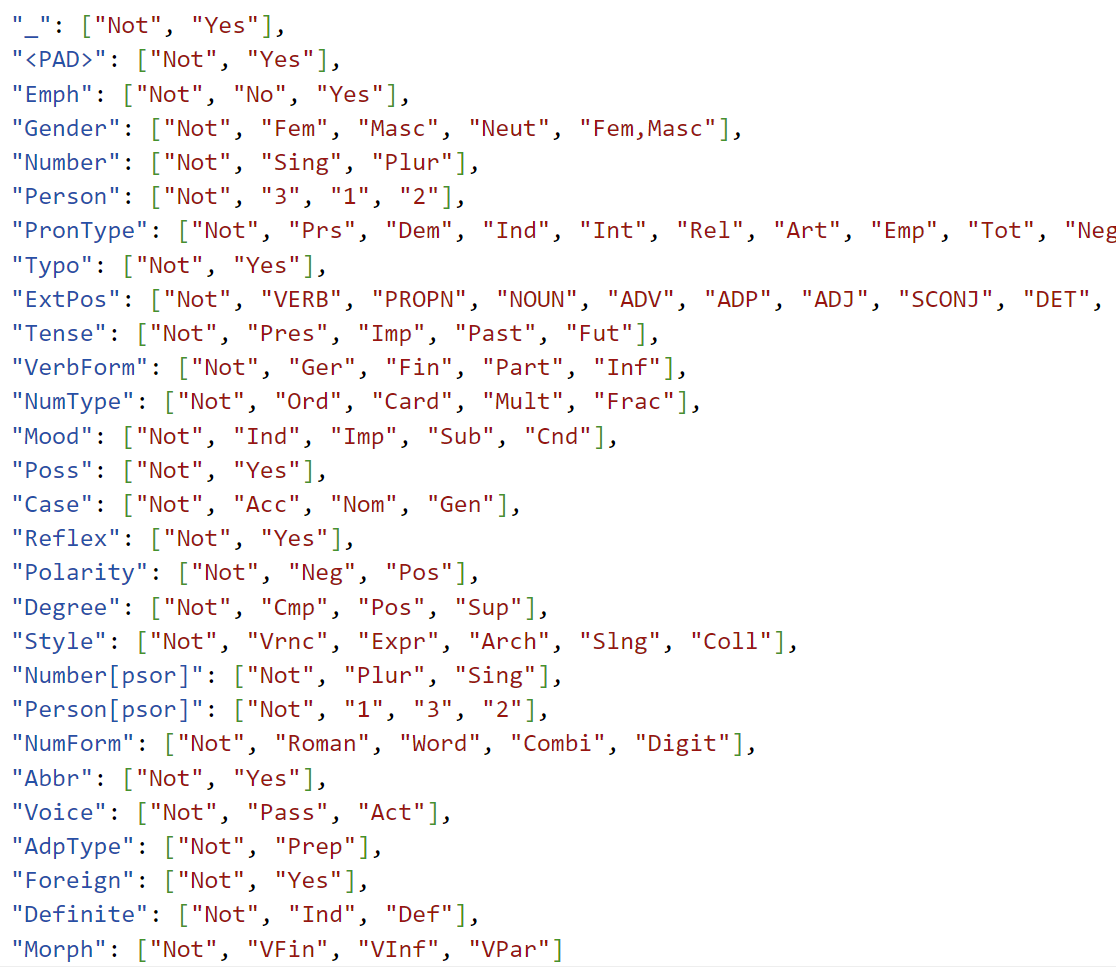
\includegraphics[width=0.8\textwidth]{all_morphy.png}
        \caption{Ensemble de tous les \textit{morphy}}
    \end{figure}
\end{frame}

\begin{frame}{Les Données: création de séquences}
    \begin{exampleblock}{Idée}
        On rajoute des caractères $\langle$PAD$\rangle$ pour compléter les phrases,
        on rajoute aussi un label qui correcponds au pad.
    \end{exampleblock}

    \bigskip
    Si on fixe une longueur de séquence à 5, on va transfomé la phrase:
    \begin{table}
        \centering
        \begin{tabular}{|c|c|c|}
            \hline
            \textbf{type} & \textbf{exemple} & \textbf{longueur} \\
            \hline
            phrase & Les poissons sont des animaux vertébrés . & 7 \\
            \hline
            sequence & Les poissons sont des animaux & 5\\
             & vertébrés . $\langle$PAD$\rangle$ $\langle$PAD$\rangle$ $\langle$PAD$\rangle$ & 5\\
            \hline
        \end{tabular}
        \caption{Exemple de la création du séquences}
    \end{table}
\end{frame}

\begin{frame}{Les Données: La gestion des mots inconnus}
    \begin{exampleblock}{Idée}
        Si le modèle rencontre un mot inconnus, il va le remplacer par le mot $\langle$UNK$\rangle$.
        Le modèle doit alors aussi apprendre ce mot lors de l'entraînement.
    \end{exampleblock}

    \begin{itemize}
        \item Avant l'entraînement, on fait un dropout des mots avec un taux d'oublie de $1\%$.
        \item On obtient un nombre de mots dans le vocabulaire de taille 67814 (contre 76048 dans le dataset).
        \item On a fixé la seed avant
    \end{itemize}
\end{frame}

\begin{frame}{Les Données: Encodage des labels}
    Pour les \textit{pos} :
    \begin{itemize}
        \item On remplace le label par son indice dans la liste des labels.
    \end{itemize}
    Pour les \textit{morphy} :
    \begin{itemize}
        \item On remplace le label par une liste d'indice, où l'éléments $i$ de la liste corresponds à l'incide du $i$-ème type de morphy.
    \end{itemize}
    Exemple: \textit{Emph=No$\mid$Number=Sing$\mid$Person=1$\mid$PronType=Prs}

    [0, 0, 1, 0, 1, 2, 9, 0, 0, 0, 0, 0, 0, 0, 0, 0, 0, 0, 0, 0, 0, 0, 0, 0, 0, 0, 0, 0]

    \begin{itemize}
        \item Entrée: $x$ de taille $B \times K$ contenant les indices des mots
        \item Sortie de \textit{pos}: $y_{pos}$ de taille $B \times K \times 19$
        \item Sortie de \textit{morphy}: $y_{morphy}$ de taille $B \times K \times 28 \times 13$
    \end{itemize}
\end{frame}

\begin{frame}{Modèle \textit{GET\_POS}}
    \begin{figure}
        \centering
        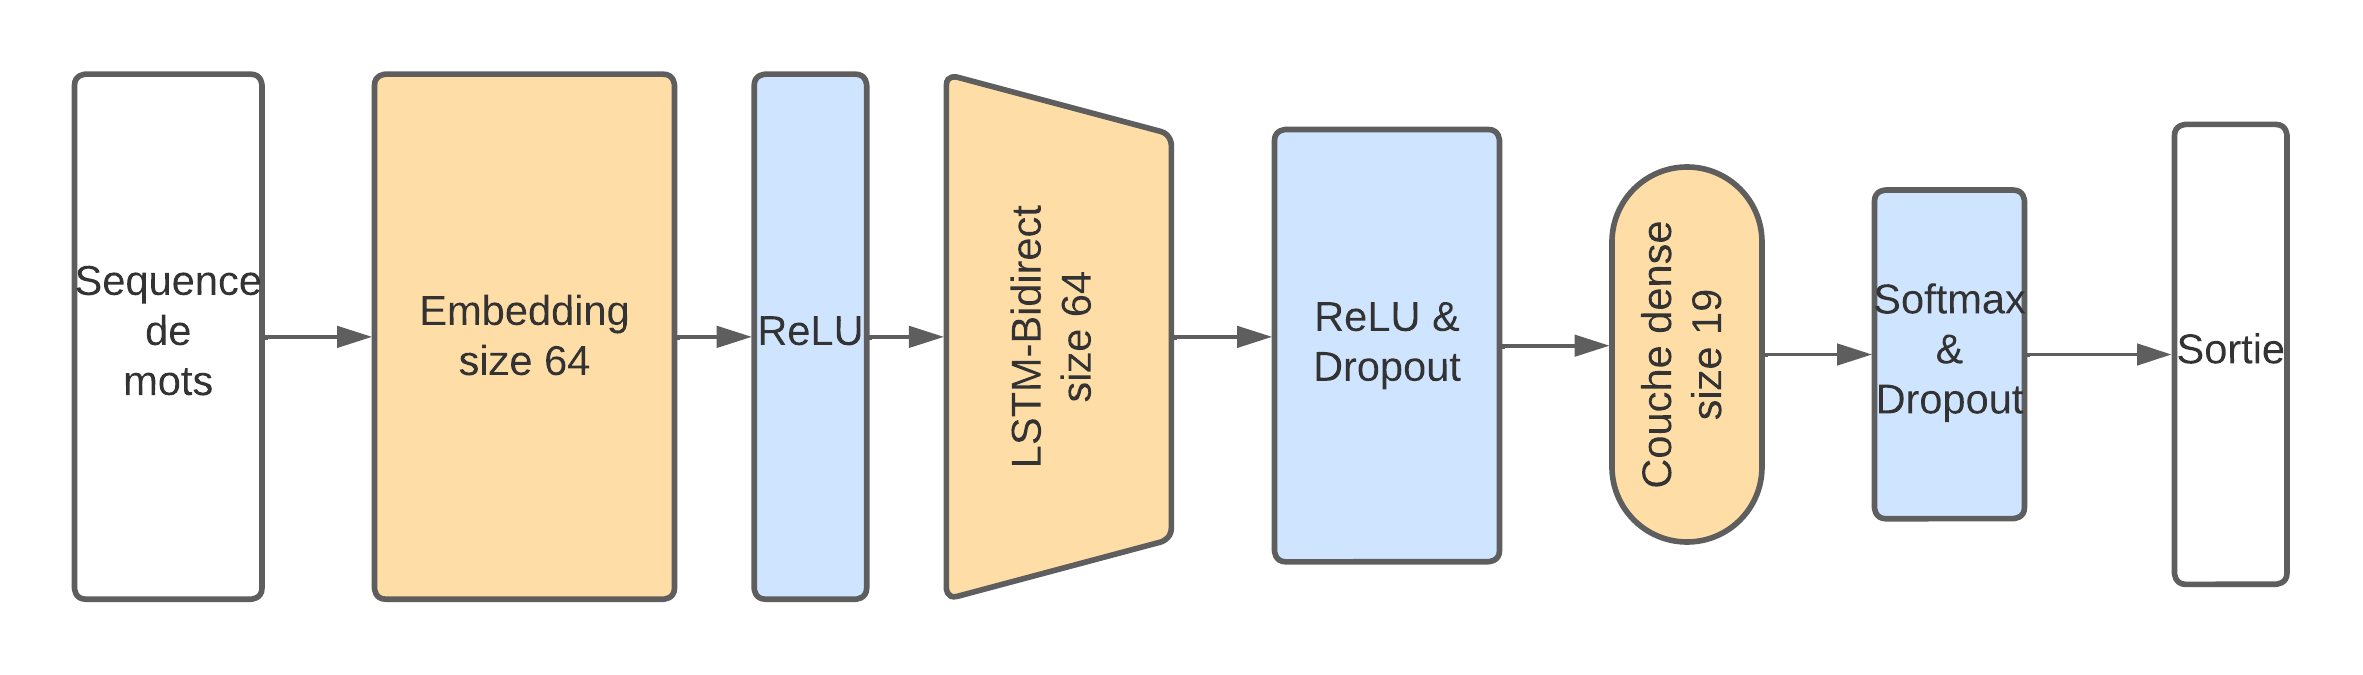
\includegraphics[width=\textwidth]{get_pos.png}
        \caption{Modèle \textit{GET\_POS}}
        \label{fig: model getpos}
    \end{figure} 
\end{frame}

\begin{frame}{Modèle \textit{SUPERTAG}}
    \begin{figure}
        \centering
        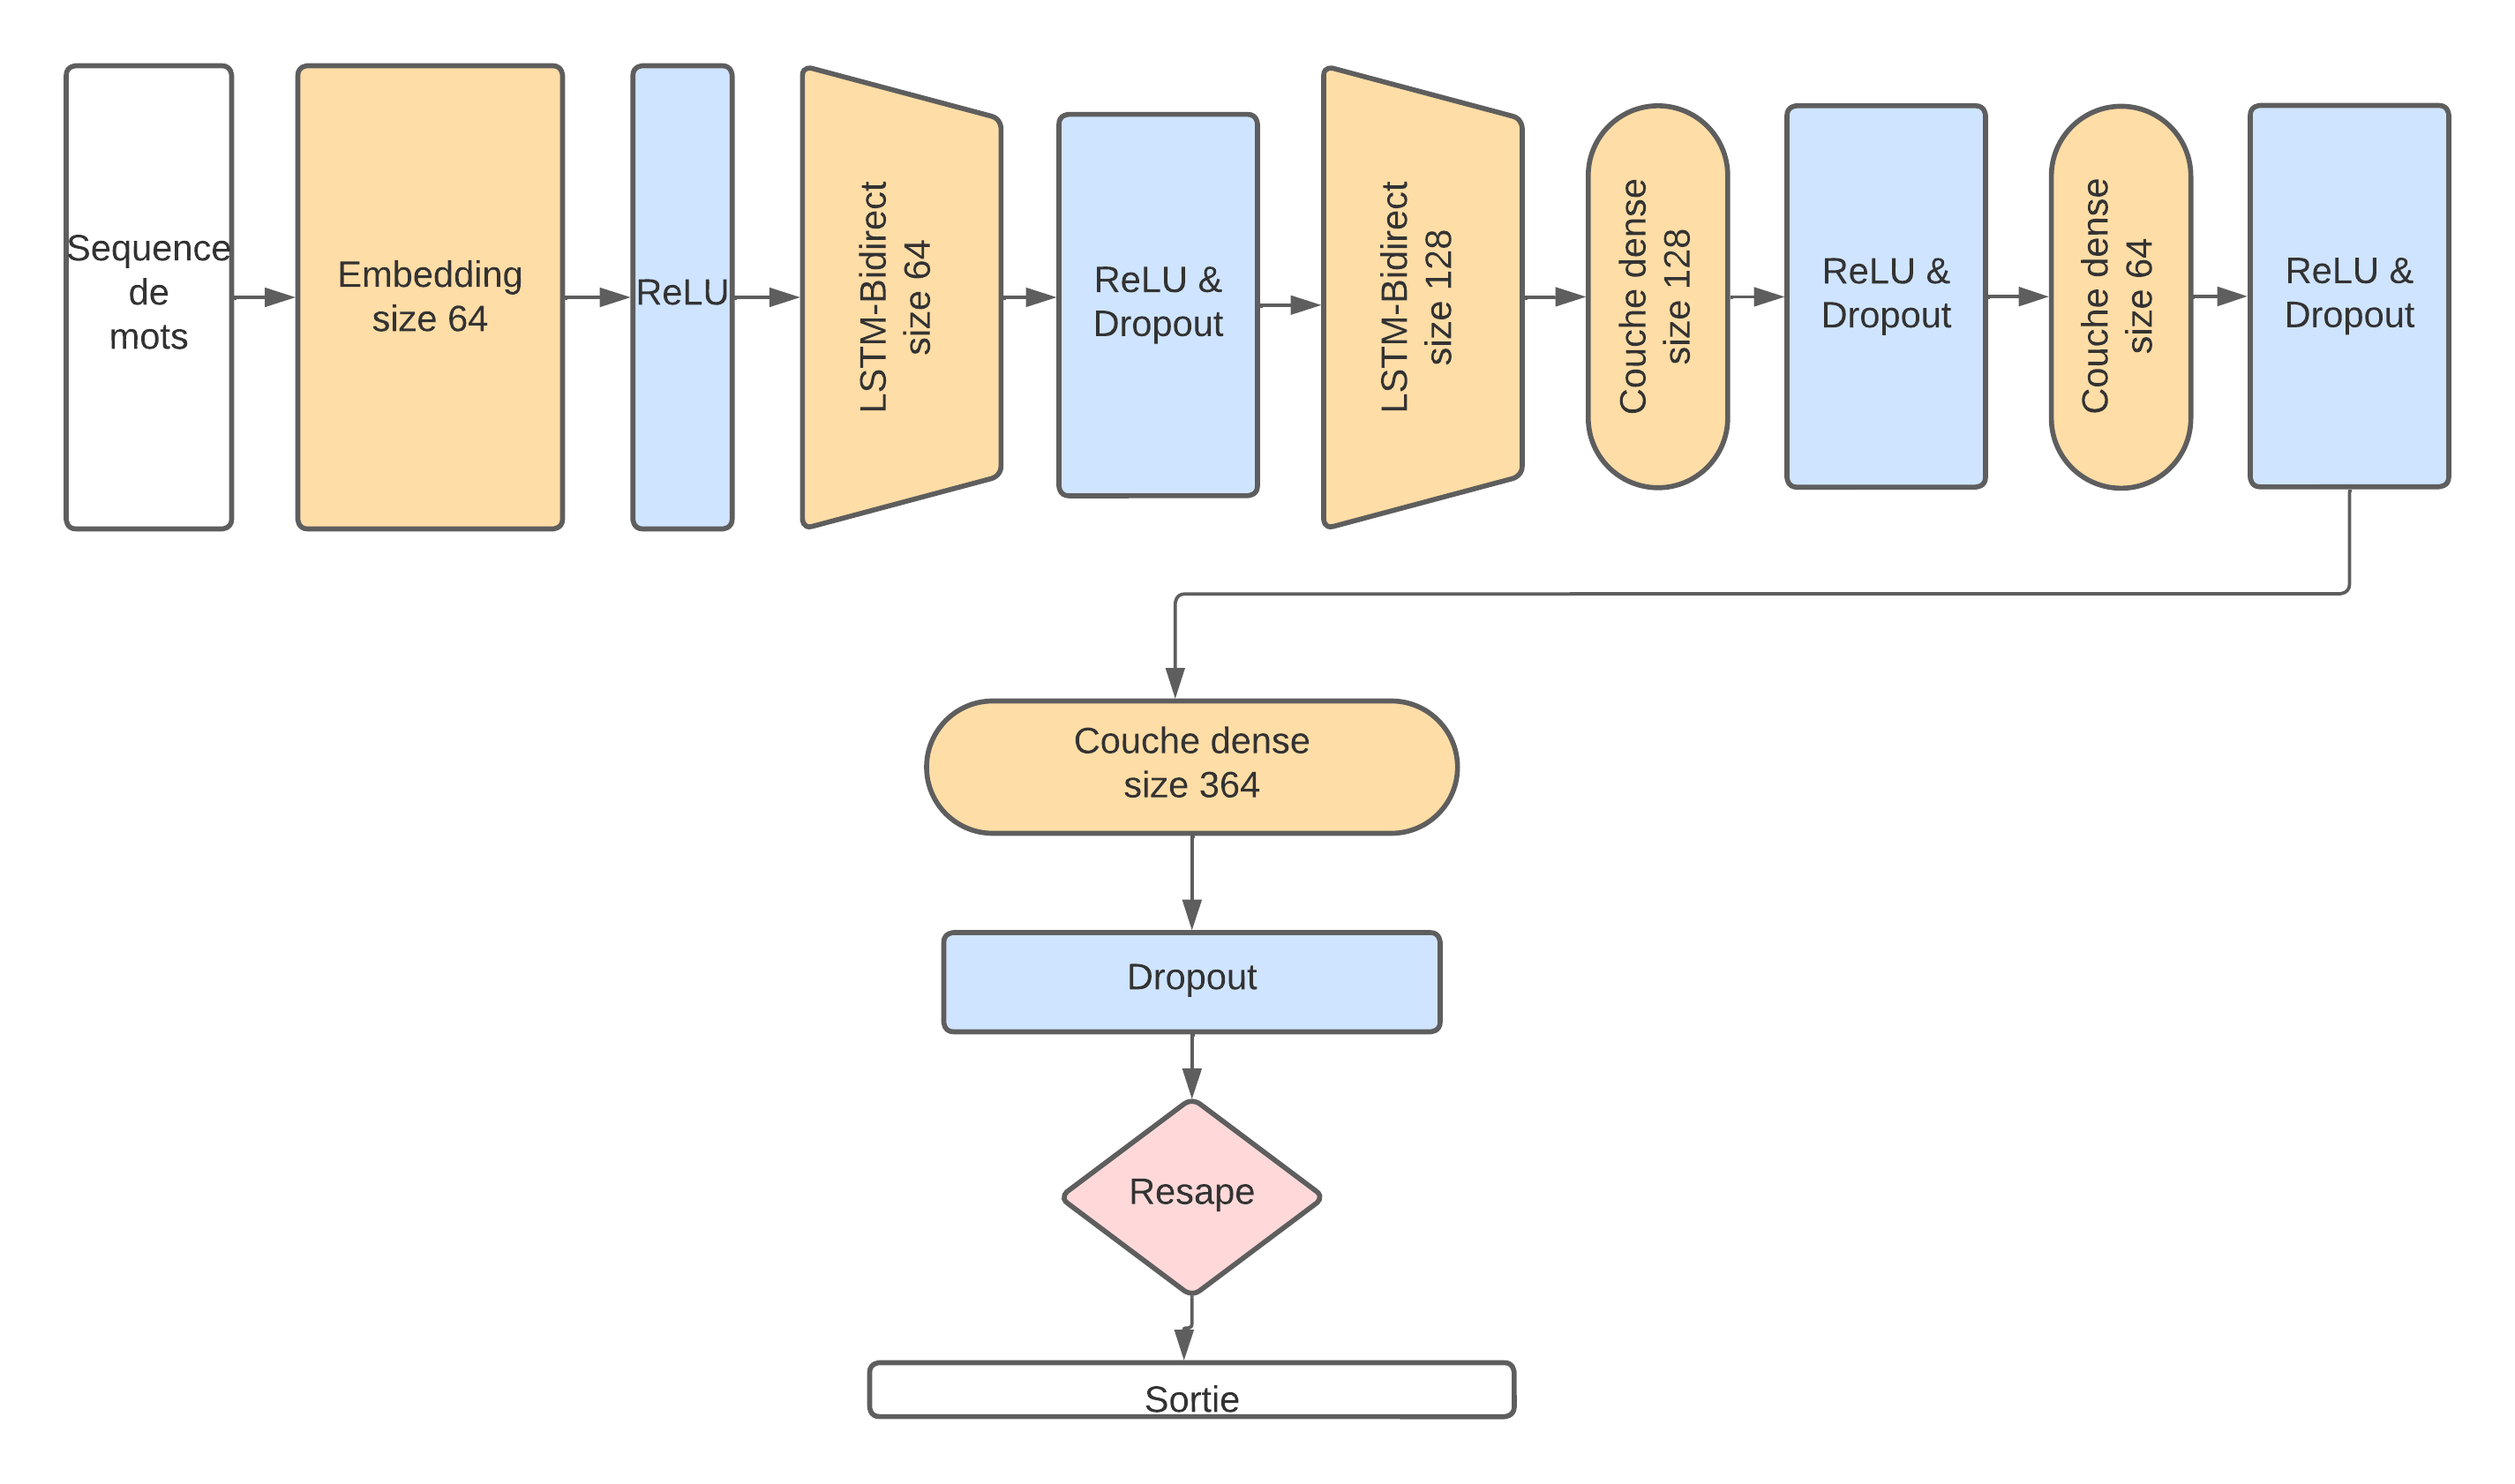
\includegraphics[width=\textwidth]{get_morphy_supertag.png}
        \caption{Modèle \textit{SUPERTAG}}
        \label{fig: model supertag}
    \end{figure}
\end{frame}

\begin{frame}{Modèle \textit{SEPARATE}}
    \begin{figure}
        \centering
        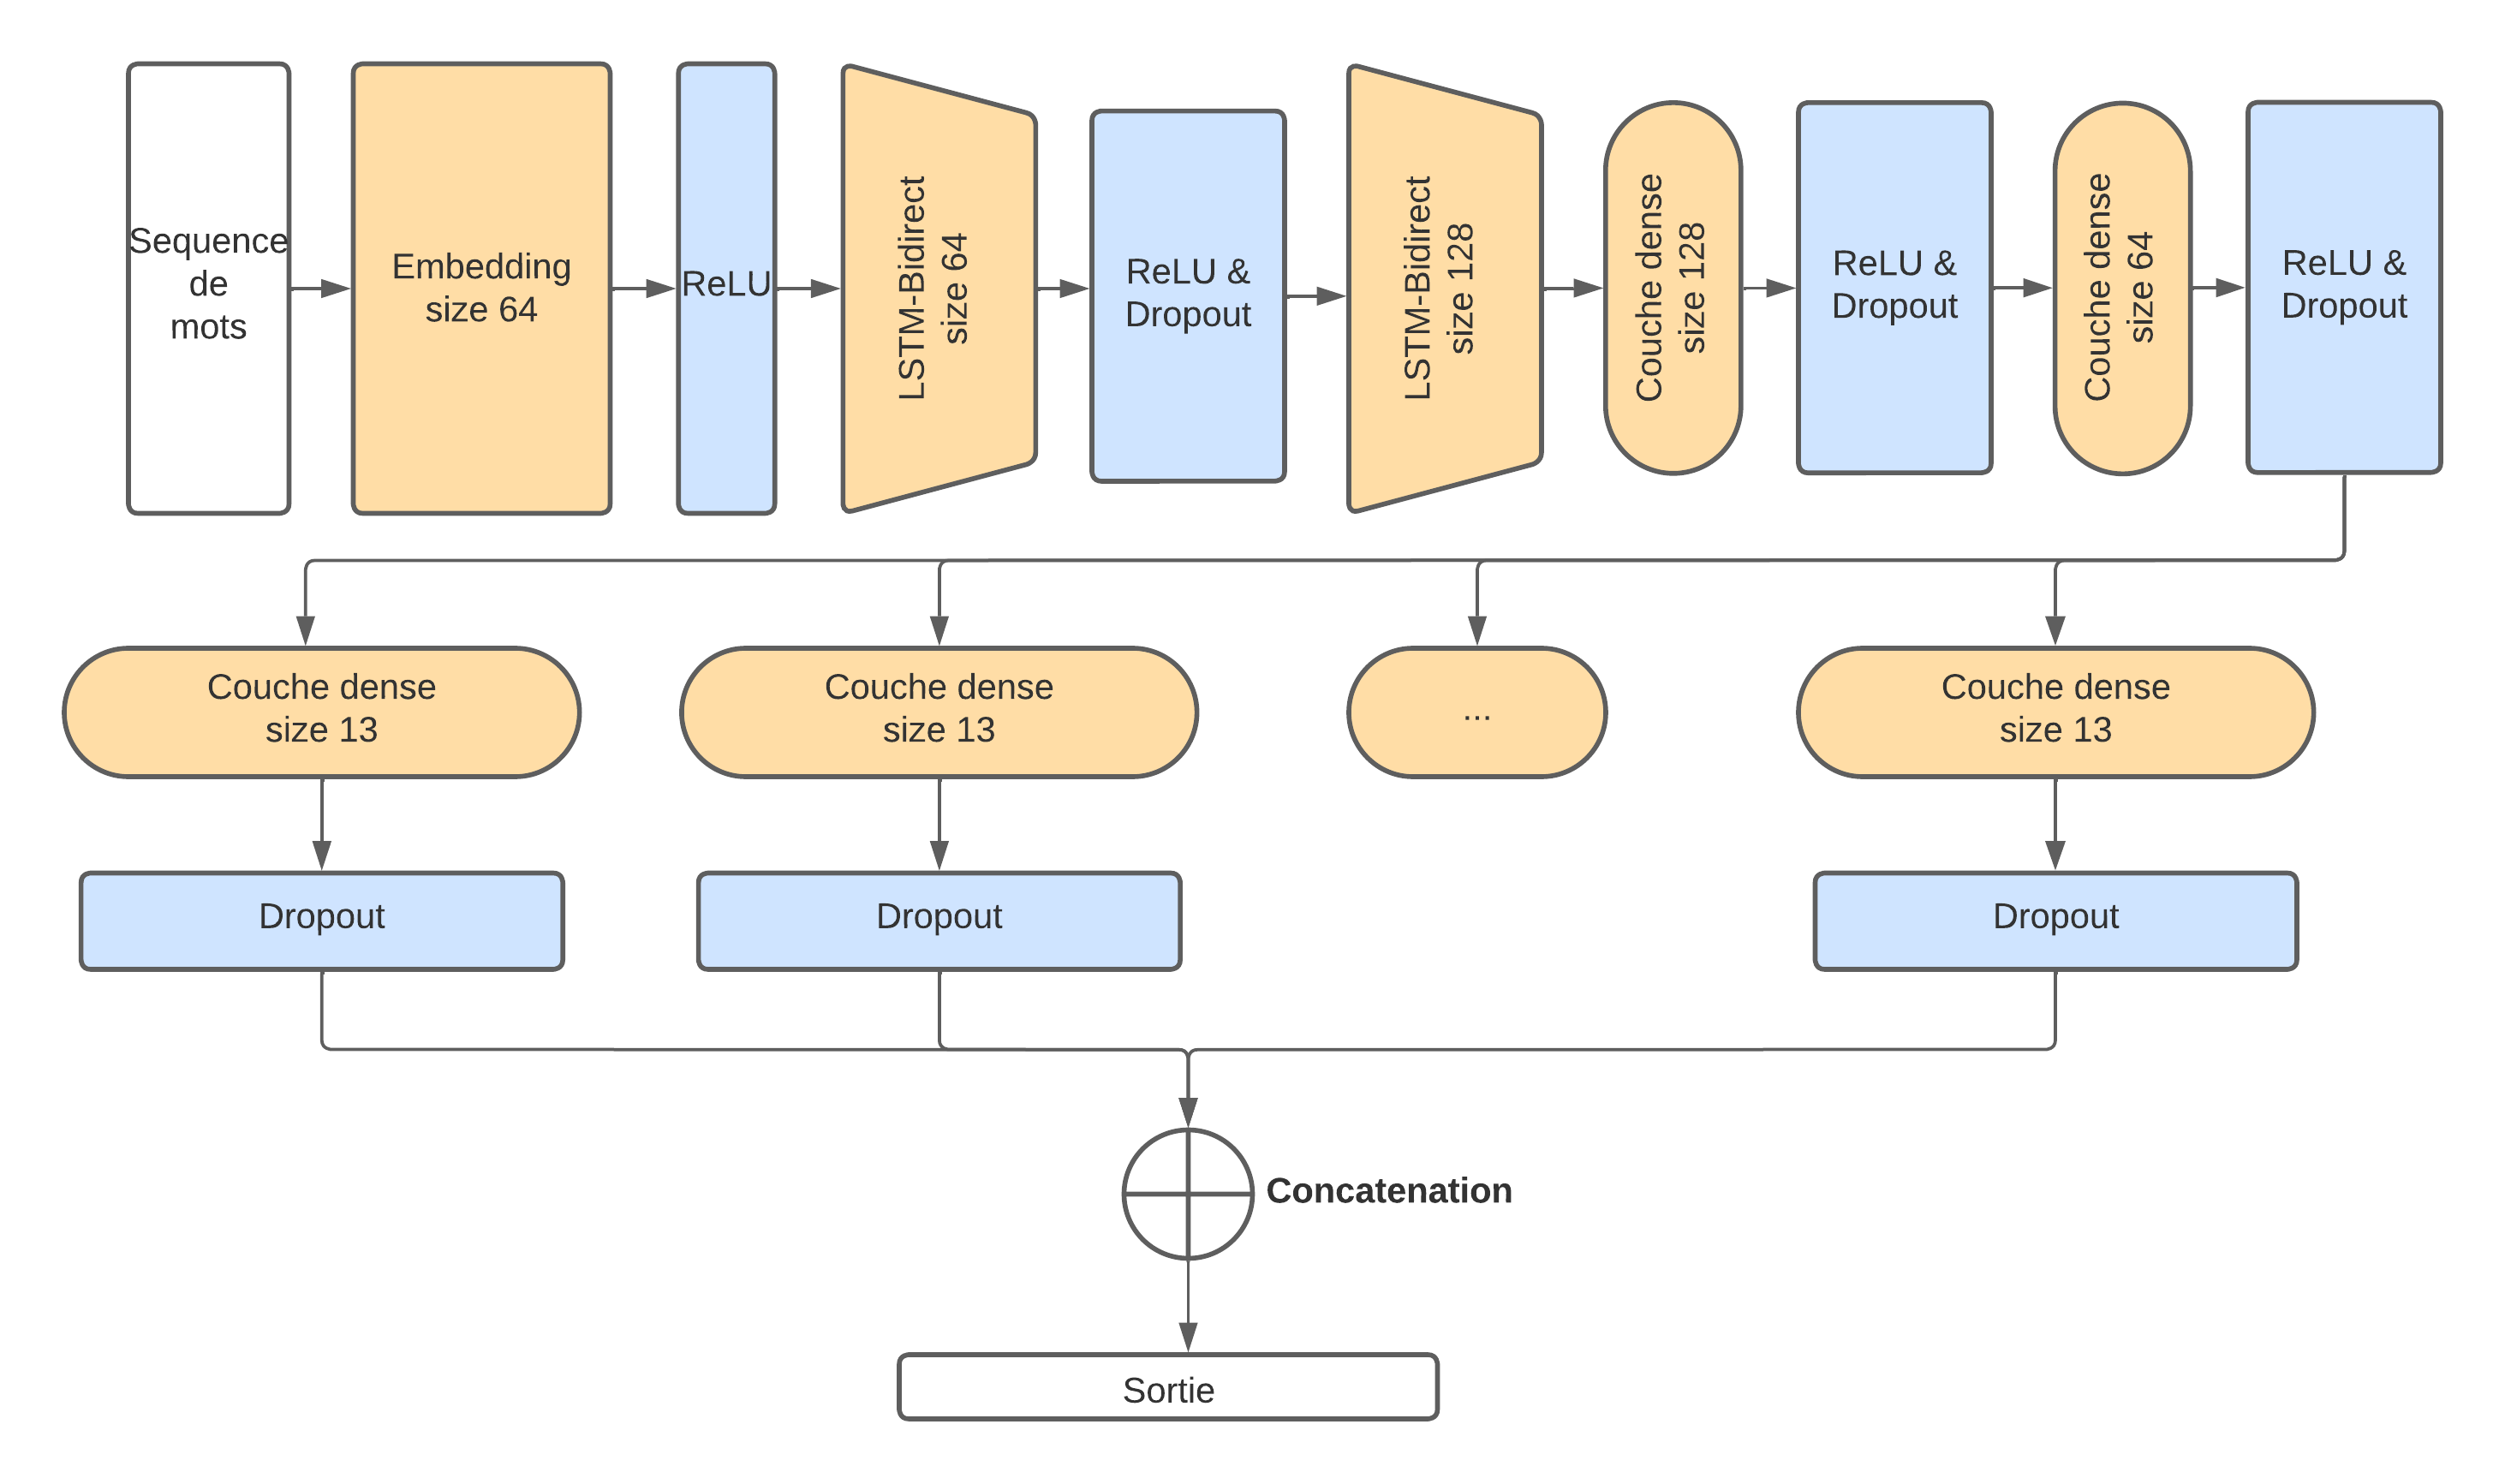
\includegraphics[width=\textwidth]{get_morphy_separate.png}
        \caption{Modèle \textit{SEPARATE}.}
        \label{fig: model separate}
    \end{figure}
\end{frame}

\begin{frame}{Modèle \textit{FUSION}}
    \begin{figure}[!ht]
        \centering
        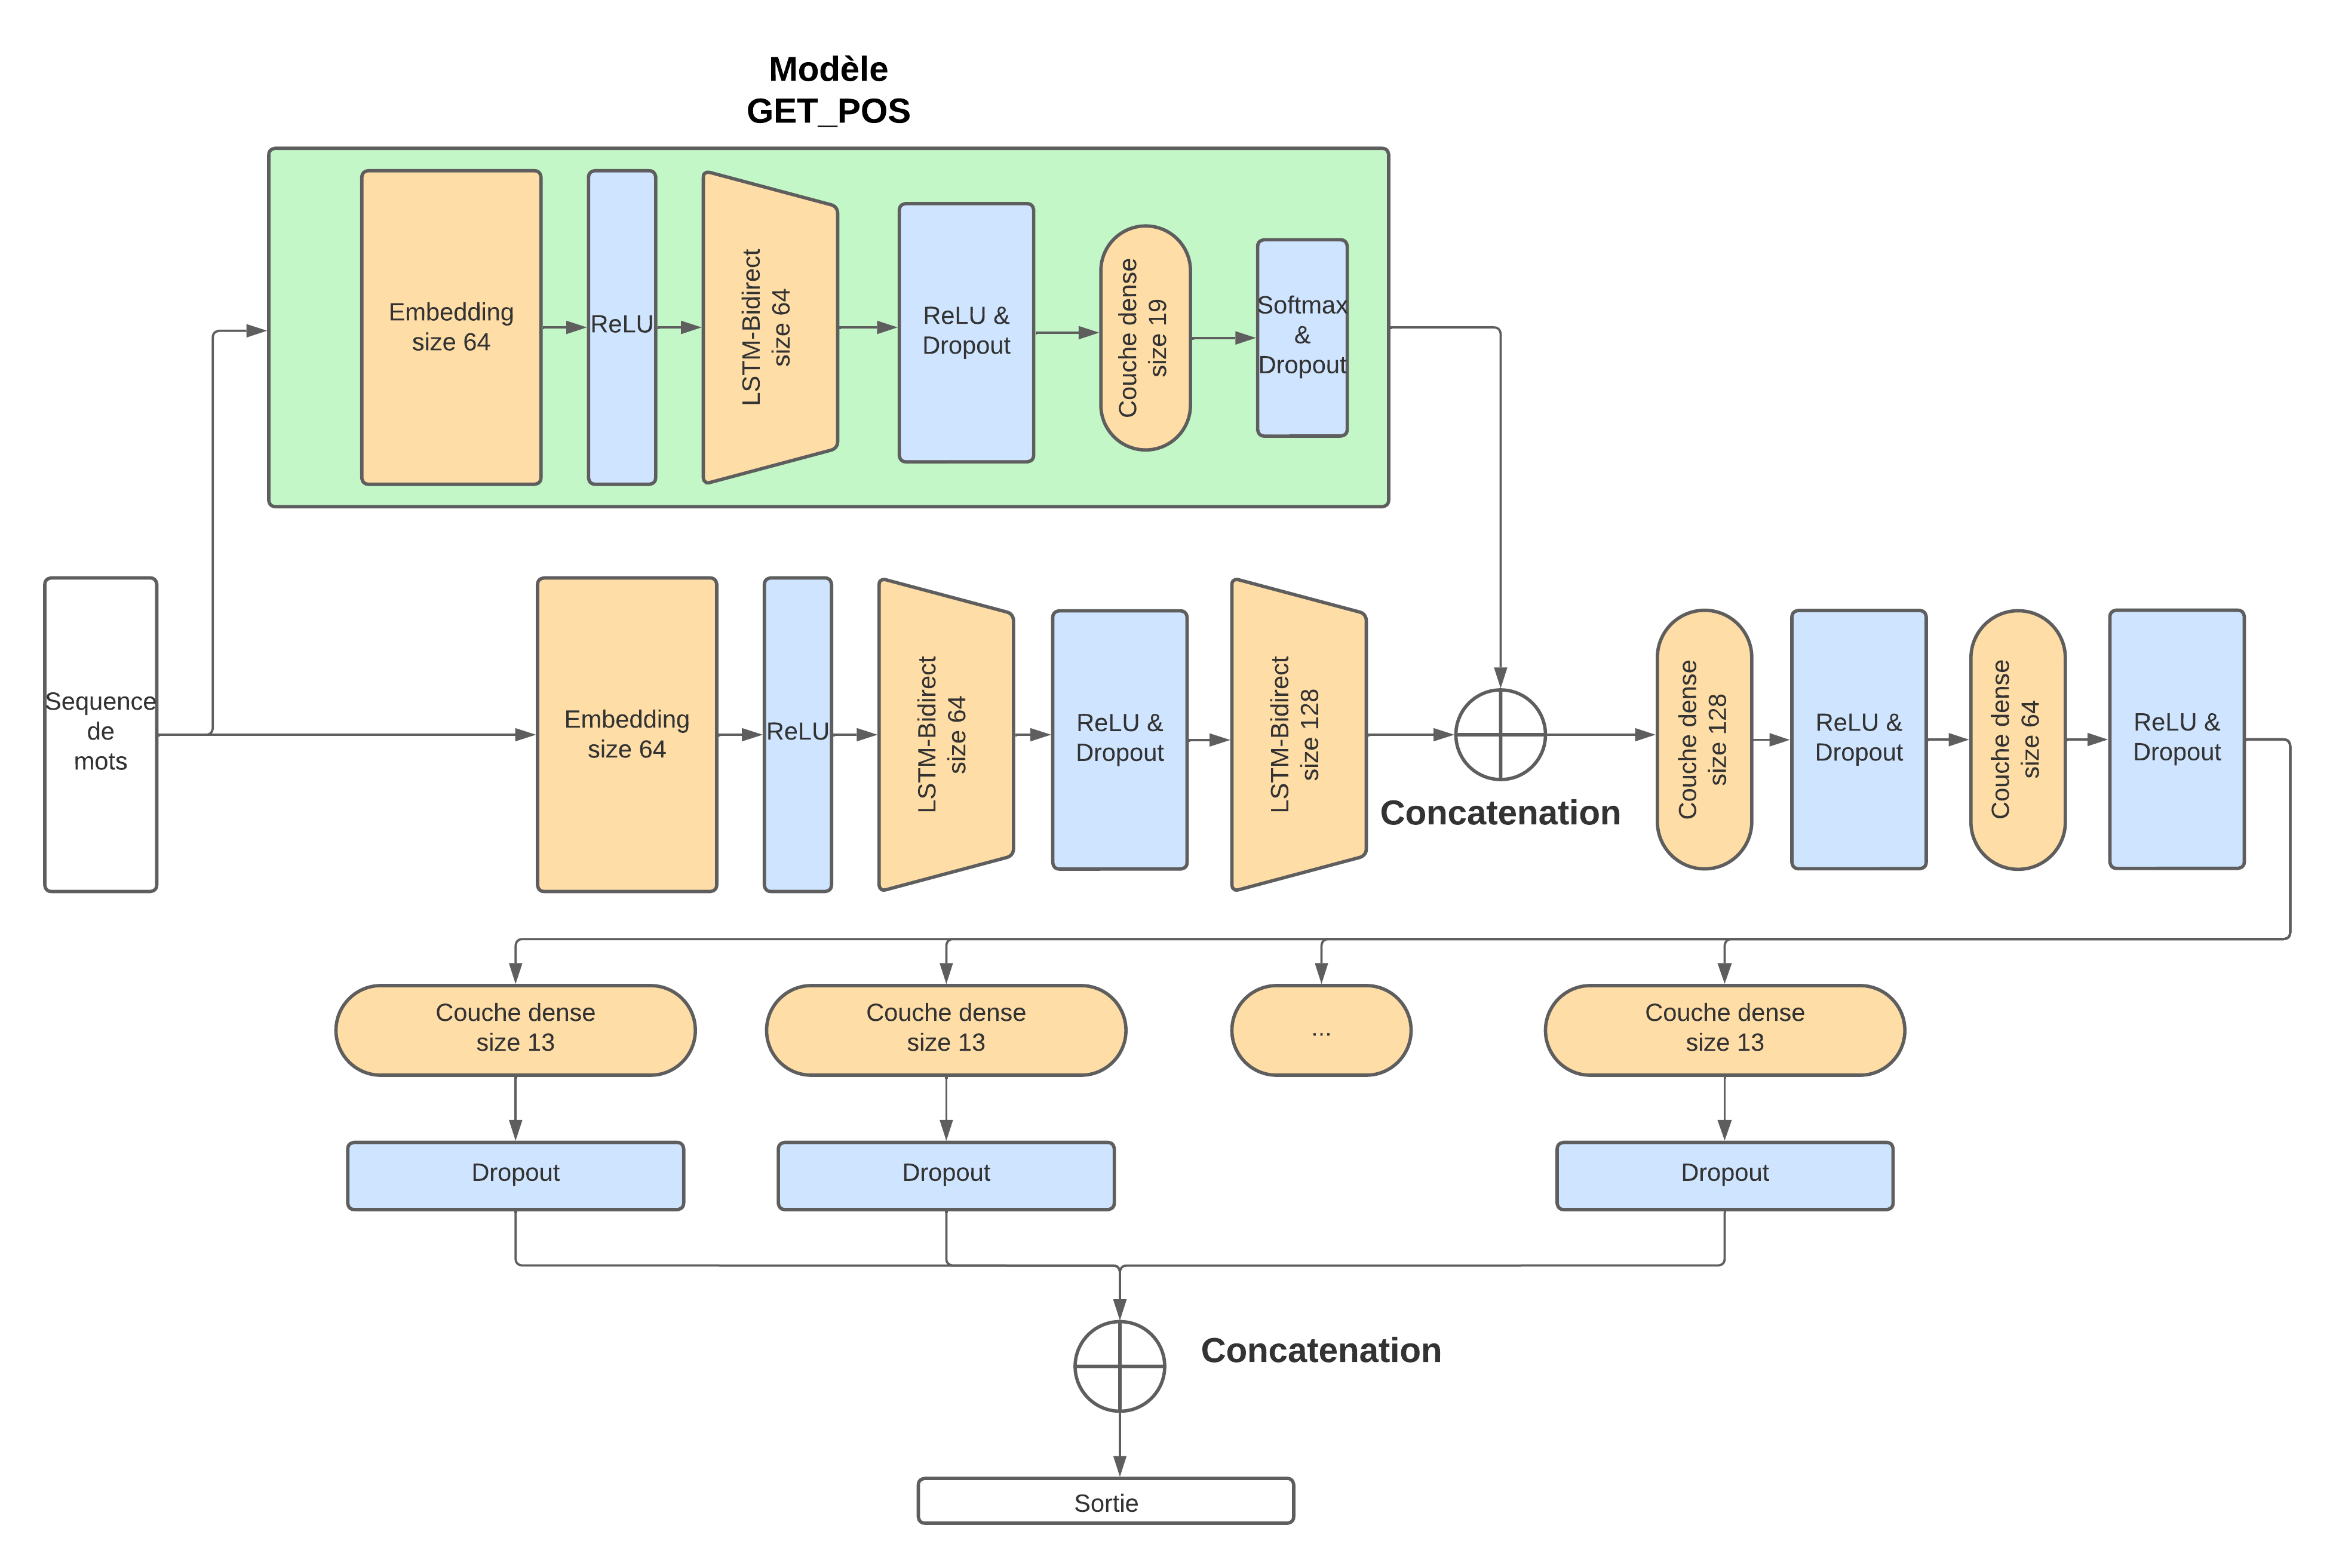
\includegraphics[width=0.9\textwidth]{get_morphy_fusion.png}
        \caption{Modèle \textit{FUSION}}
        \label{fig: model fusion}
    \end{figure}
\end{frame}

\begin{frame}{Loss et Métriques}
    Les loss:
    \begin{itemize}
        \item crossentropy pour le \textit{pos}
        \item moyenne de la crossentropy sur les 28 classes pour le \textit{morphy}
    \end{itemize}
    Les métriques:
    \begin{itemize}
        \item accuracy micro
        \item accuracy macro (pour le \textit{pos})
        \item allgood (pour le \textit{morphy})
    \end{itemize}
\end{frame}

\begin{frame}{Résultats: \textit{GET\_POS} }
    \begin{figure}
        \centering
        \begin{subfigure}{0.32\textwidth}
            \centering
            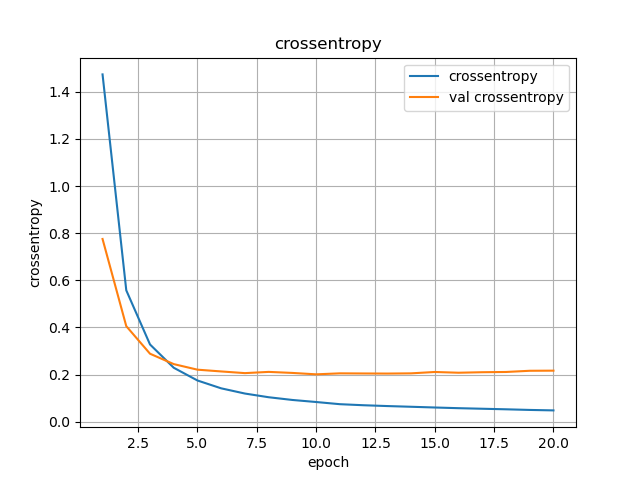
\includegraphics[width=\linewidth]{../logs/get_pos_French/crossentropy.png}
        \end{subfigure}
        \begin{subfigure}{0.32\textwidth}
            \centering
            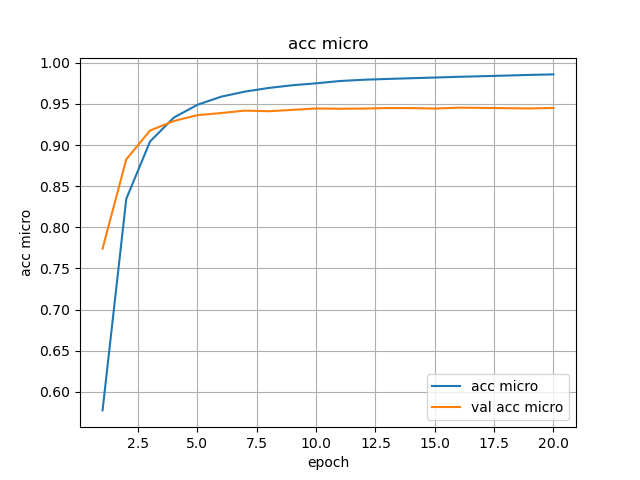
\includegraphics[width=\linewidth]{../logs/get_pos_French/acc micro.png}
        \end{subfigure}
        \begin{subfigure}{0.32\textwidth}
            \centering
            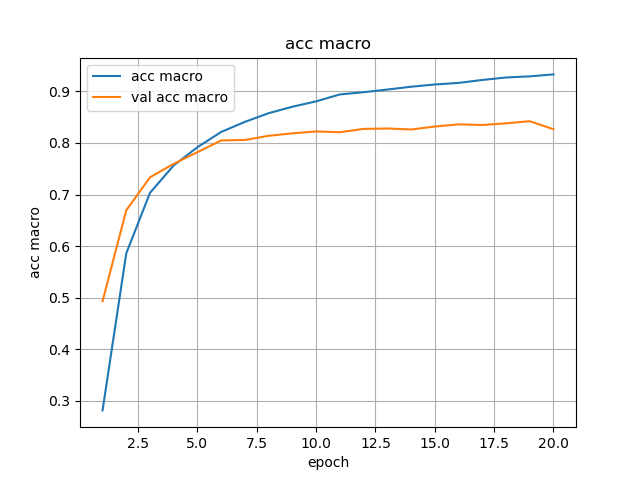
\includegraphics[width=\linewidth]{../logs/get_pos_French/acc macro.png}
        \end{subfigure}
        \caption{Entraînement du modèle \textit{GET\_POS}.}
    \end{figure}

    \begin{table}
        \centering
        \begin{tabular}{|c|c|c|c|}
            \hline
            Nom du modèle & crossentropy & accuracy micro & accuracy macro \\
            \hline
            \textit{GET\_POS} & 0.204 & 0.944 & 0.816\\
            \hline
        \end{tabular}
        \caption{Résultats du modèle \textit{GET\_POS} sur la base de données de teste.}
        \label{tab:test getpos}
    \end{table}
\end{frame}

\begin{frame}{Résultats des modèles \textit{SUPERTAG} et \textit{SEPARATE}}
    \begin{figure}
        \centering
        \begin{subfigure}{0.32\textwidth}
            \centering
            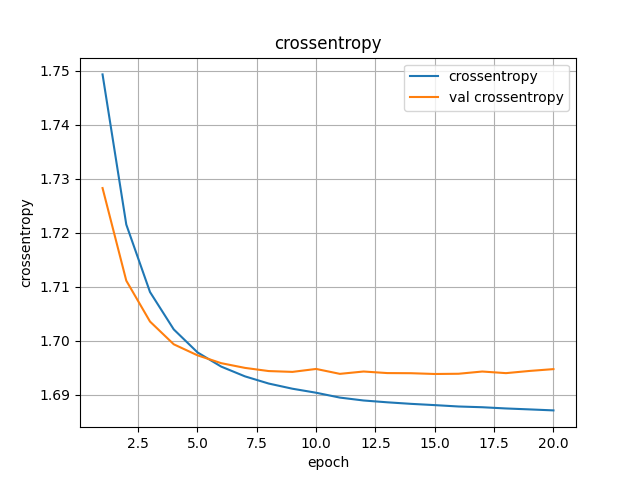
\includegraphics[width=\linewidth]{../logs/supertag/crossentropy.png}
        \end{subfigure}
        \begin{subfigure}{0.32\textwidth}
            \centering
            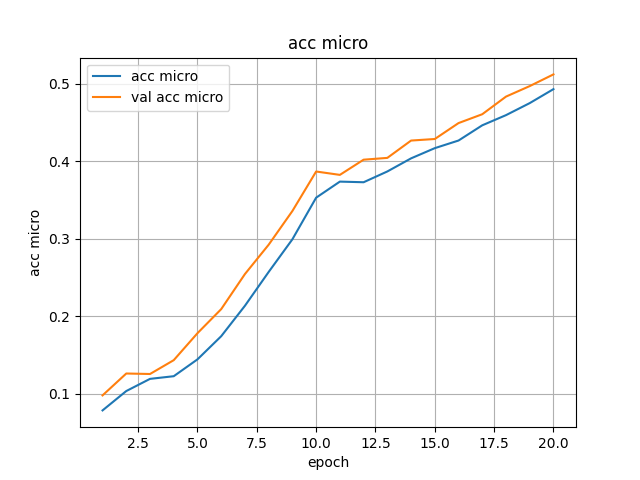
\includegraphics[width=\linewidth]{../logs/supertag/acc micro.png}
        \end{subfigure}
        \begin{subfigure}{0.32\textwidth}
            \centering
            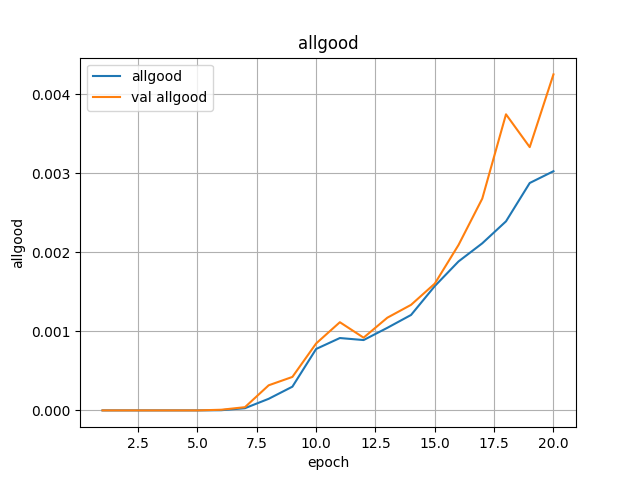
\includegraphics[width=\linewidth]{../logs/supertag/allgood.png}
        \end{subfigure}
        \caption{Entraînement du modèle \textit{SUPERTAG}.}
        \label{fig: results supertag}
    \end{figure}
    \begin{figure}
        \centering
        \begin{subfigure}{0.32\textwidth}
            \centering
            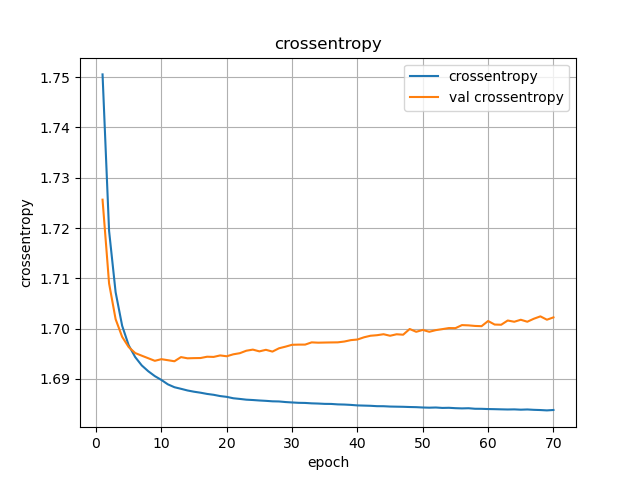
\includegraphics[width=\linewidth]{../logs/separate/crossentropy.png}
        \end{subfigure}
        \begin{subfigure}{0.32\textwidth}
            \centering
            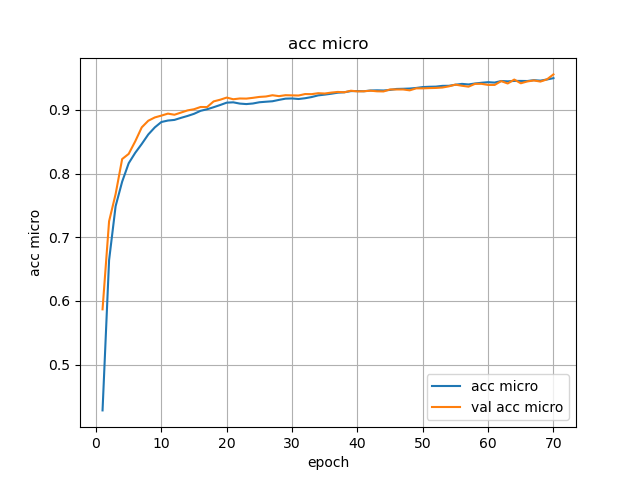
\includegraphics[width=\linewidth]{../logs/separate/acc micro.png}
        \end{subfigure}
        \begin{subfigure}{0.32\textwidth}
            \centering
            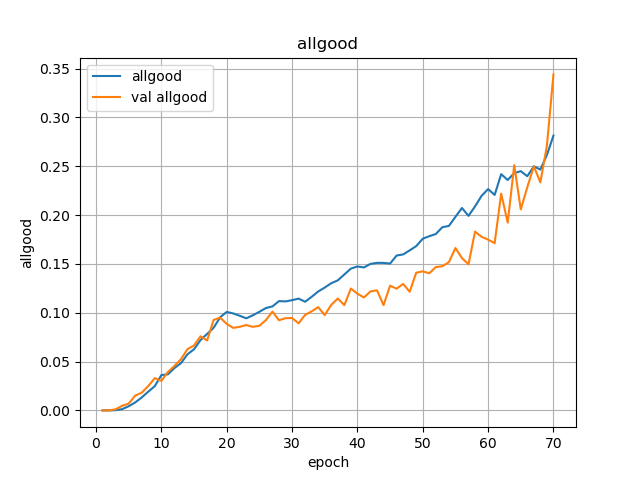
\includegraphics[width=\linewidth]{../logs/separate/allgood.png}
        \end{subfigure}
        \caption{Entraînement du modèle \textit{SEPARATE}.}
        \label{fig: results separate}
    \end{figure}
\end{frame}

\begin{frame}{Résultats du modèle \textit{FUSION} et résultats de teste}
    \begin{figure}
        \centering
        \begin{subfigure}{0.32\textwidth}
            \centering
            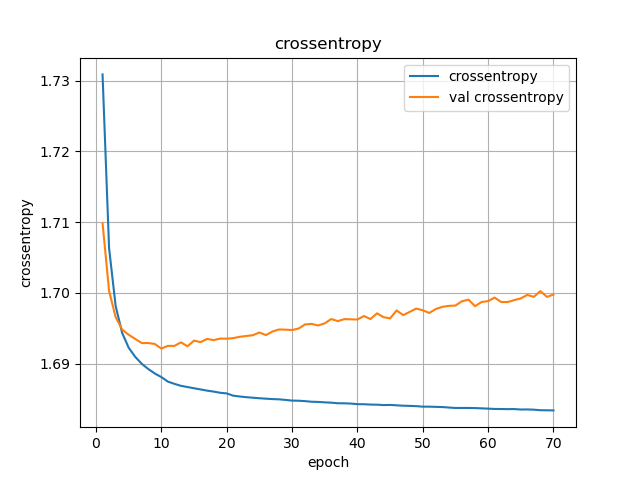
\includegraphics[width=\linewidth]{../logs/fusion/crossentropy.png}
        \end{subfigure}
        \begin{subfigure}{0.32\textwidth}
            \centering
            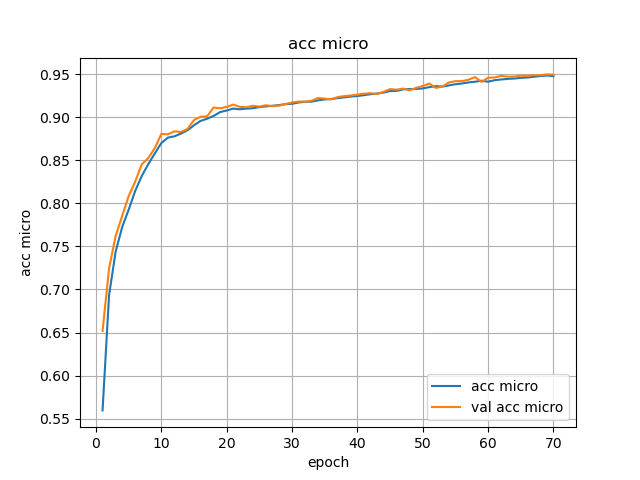
\includegraphics[width=\linewidth]{../logs/fusion/acc micro.png}
        \end{subfigure}
        \begin{subfigure}{0.32\textwidth}
            \centering
            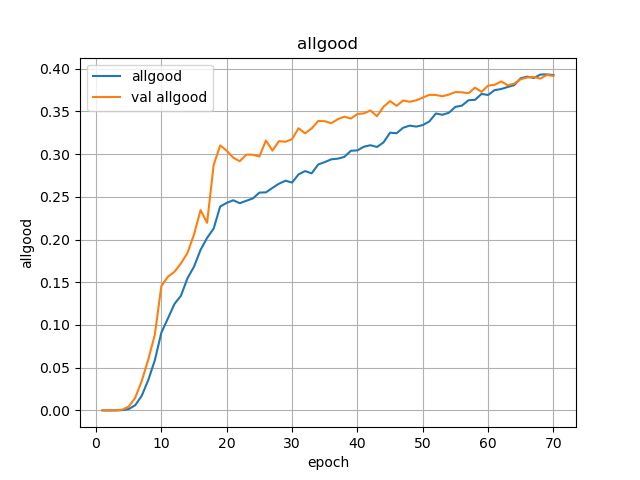
\includegraphics[width=\linewidth]{../logs/fusion/allgood.png}
        \end{subfigure}
        \caption{Entraînement du modèle \textit{FUSION}.}
        \label{fig: results fusion}
    \end{figure}

    \begin{table}
        \centering
        \begin{tabular}{|c|c|c|c|}
            \hline
             Nom du modèle & crossentropy & accuracy micro & all good\\
             \hline
             \textit{BASELINE}& - & 0.980 & 0.791 \\
             \hline
             \textit{SUPERTAG}& 1.700 & 0.436 & 0.002\\
             \hline
             \textit{SEPARATE}& 1.70 & 0.893 & 0.046\\
             \hline
             \textit{FUSION}& 1.698 & 0.884 & 0.154 \\
             \hline
        \end{tabular}
        \caption{Résultats de test sur la prédiction des \textit{morphy}}
        \label{tab: test morphy}
    \end{table}
\end{frame}

\begin{frame}
    
\end{frame}

\begin{frame}
    
\end{frame}

\begin{frame}
    
\end{frame}





\end{document}

